% \section{Introduction}
\clearpage

% Recommender systems aim to recover users’ latent interests from their past interactions. Inspired by the rapid progress of generative models—especially large language models (LLMs) \cite{GPT3,gpt4,qwen2.5,deepseek}—the community has begun to recast recommendation as a generative task. Under this paradigm, known as generative recommendation \cite{TIGER,LCRec,TOKENRec,OneRec,mtgr}, the model directly produces a sequence of item identifiers in an autoregressive fashion, replacing the conventional score-then-rank pipeline. 
% Representing items with Semantic IDs (SIDs) lets the generative recommender share parameters across semantically related items, cover billion-scale catalogs with a compact vocabulary, and naturally align with the hierarchical reasoning style of LLMs.

The powerful sequence modeling capabilities of large language models (LLMs) have enabled their adaptation to recommender systems \citep{BIGRec, AlphaRec, AlphaFuse, LLM2REC, survey_LLM_Rec, survey_seq}, with generative recommendation emerging as a promising direction that leverages autoregressive generation for item prediction \citep{TIGER, LCRec, TOKENRec, HSTU, OneRec, mtgr}.
% This paradigm centers on generating sequences of Semantic IDs (SIDs)---discrete tokens that encode item semantics through quantization of continuous embeddings \citep{rqvae, rqkmeans}.
% By promoting token sharing across semantically related items, SIDs facilitate efficient handling of large-scale catalogs while naturally aligning with the step-by-step (chain-of-thought) reasoning paradigm of LLMs \citep{TIGER, rqvae, rqkmeans, OneRec, bettersid}.
\kxy{Notably, unlike Large Embedding Models~(LEMs) that devote the majority of their parameters to embedding tables, OneRec\citep{OneRec} shows that increasing network depth is an effective way to learn Semantic IDs~(SIDs)—discrete tokens that represent item semantics through the quantization of continuous embeddings~\citep{rqvae,rqkmeans}. To a certain extent, this finding corroborates the emerging scaling law in recommendation: deeper networks, while keeping the vocabulary size compact, can absorb richer semantic signals and consequently yield noticeably better recommendation performance.}


Upon scrutinizing prior studies on generative recommenders, we can summarize a common \za{training} pipeline:
(1) \za{Beginning with items'} textual descriptions or embeddings, a quantization method transforms continuous vectors into SIDs.
(2) The model is then trained to generate these SIDs in an end-to-end \za{manner, typically following} two primary approaches: \textit{scratch-trained recommenders} that train Transformer \citep{Transformer} from scratch on user interaction sequences \citep{TIGER, HSTU, OneRec, mtgr}, and \textit{SID-aligned Recommenders} that adapt pretrained LLMs \za{from the language space into SID space} through supervised fine-tuning (SFT) \citep{LCRec, TOKENRec}.
\za{Although these methods achieve promising performance, the integration of reinforcement learning (RL) for deeper alignment with user interaction sequences remains relatively underexplored \citep{sdpo}.} 

\za{
Inspired by the recent success of the \textbf{SFT-then-RL} paradigm \citep{deepseekmath, SFT-then-RL, o1}, we aim to establish a generative recommendation framework that adapts this paradigm to the unique characteristics of recommendation tasks. 
Specifically, we first explore applying Group Relative Policy Optimization (GRPO) \citep{Deepseek-r1} after the initial SFT phase, considering both scratch-trained and SID-aligned recommenders.
Our preliminary experiments (\cf Figure \ref{fig:sft_vs_rl}) demonstrate the effectiveness of the SFT-then-GRPO paradigm in generative recommendation, consistently outperforming the SFT-only baselines.
Building on this, we further investigate two critical limitations that arise when directly transferring the standard SFT-then-RL paradigm to recommendation, which constrain its full potential in this domain:
}

% Recently, the \textbf{SFT-then-RL} post-training paradigm has shown promise for generative models \citep{deepseekmath, Deepseek-r1, SFT-then-RL, o1}.
% Following this trend, we first explore applying this approach to generative recommenders by incorporating Group Relative Policy Optimization (GRPO) \citep{Deepseek-r1} after the initial SFT phase.
% Our preliminary experiments (\cf Figure \ref{fig:sft_vs_rl}) confirm the effectiveness of this paradigm, showing consistent improvements over SFT-only baselines.

% However, upon deeper investigation, we identify two critical limitations in directly adapting the standard SFT-then-RL approach that constrain its full potential:

% ======================


% Upon scrutinizing previous studies on generative recommenders, we can summarize a common pipeline:
% (1) Starting from the text of an item—or an embedding from another modality—then apply a quantization method to turn the continuous vector into an ordered list of code words, called SIDs.
% (2) A model is then trained to generate these semantic IDs in an end-to-end fashion. There are two major variants:
% \begin{enumerate}[label=(\alph*),leftmargin=1.5em]
% \item \textbf{Scratch-trained Recommender:} a Transformer is pre-trained from scratch on user-interaction sequences composed of SIDs \citep{TIGER, OneRec, mtgr}.
% \item \textbf{SID-aligned Recommender:} a pre-trained LLM is aligned with the item representation space through supervised fine-tuning (SFT) \citep{LCRec, TOKENRec}.
% \end{enumerate}
% (3) At inference time, the model uses beam search together with constrained decoding to generate valid SID sequences.

% Recently, the \textbf{SFT-then-RL} paradigm has proven highly effective for generative models \citep{deepseekmath, Deepseek-r1, SFT-then-RL, o1}. In this work, we first follow the LLM-based training pipeline: we perform SFT to align LLM with the item representation space, and then apply the Group relative policy optimization (GRPO) algorithm to raise the performance ceiling further. 
% As illustrated in Figure \ref{fig:sft_vs_rl}, the SFT-then-RL paradigm has surpassed the earlier SFT-only approach in generative recommendation. 
% Although this two-stage strategy represents meaningful progress, it still suffers from several limitations:

 \begin{figure*}[t]
  \centering
  \begin{subfigure}[t]{0.34\textwidth}
    \centering
    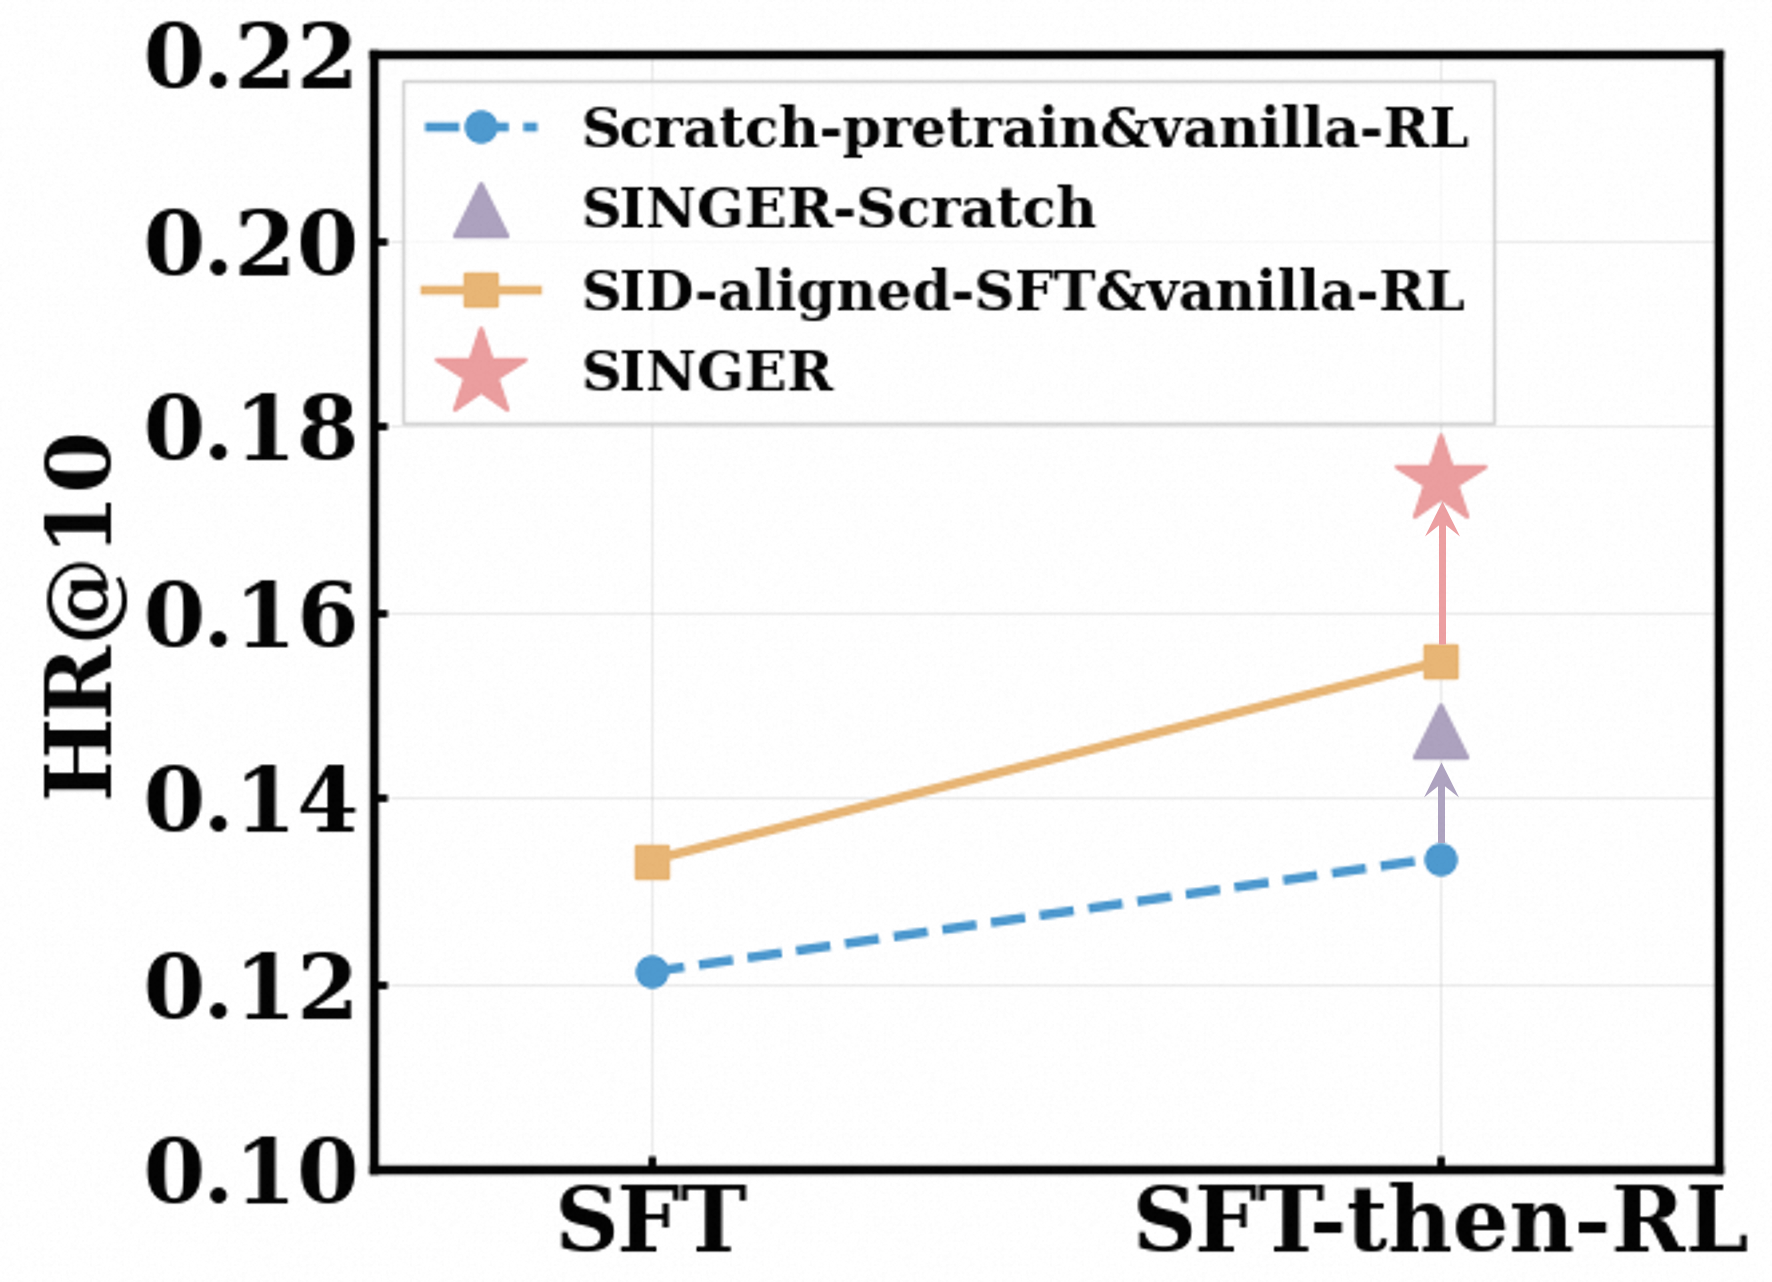
\includegraphics[width=\textwidth]{figures/sft_vs_sft_rl.png}
    \caption{Performance under Different Training Paradigms.}
    \label{fig:sft_vs_rl}
\end{subfigure}\hspace{2mm}
\begin{subfigure}[t]{0.43\textwidth}
    \centering
    \raisebox{15pt}{% 
        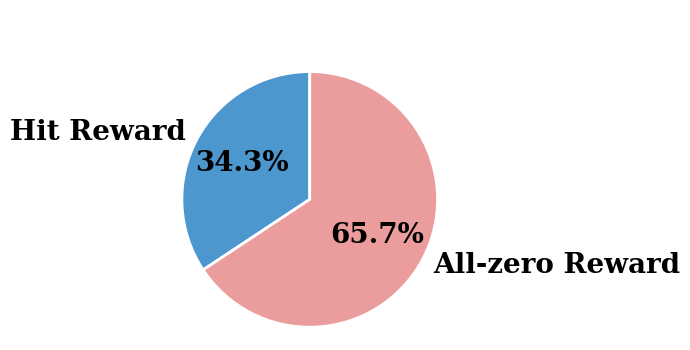
\includegraphics[width=\textwidth]{figures/pie.png}}
    \caption{Sample hit reward distribution.}
    \label{fig:pie}
\end{subfigure}
  \caption{Results on the Industrial dataset. Figure \ref{fig:sft_vs_rl} illustrates the performance, with respect to HitRatio@10 under different training paradigms. Figure \ref{fig:pie} shows the proportion of RL-sampled outputs from the SFT-initialized model that receive a non-zero reward.}
  \label{fig:teaser}
    \vspace{-10pt}
\end{figure*}


\begin{itemize}[leftmargin=*]
    % \item \textbf{Superficial SID understanding via world knowledge.}
    \label{llmmatter}
    \item \textbf{Limited SID Understanding in Alignment}.
    The SFT alignment process \za{constrains} LLMs to project outputs \za{into a closed SID vocabulary} through supervised training on user-item interaction sequences. 
    Such rigid constraint \za{mainly encourages superficial pattern matching rather than true semantic understanding of SIDs.}
    As illustrated in Figure \ref{fig:superficial_align}, even after \za{SFT the model often fails to exploit SID histories correctly: it either resorts to generic responses citing insufficient user information, or produces} lengthy, repetitive item descriptions \za{indicative of collapsed generation.}
    %when presented with SID-formatted interaction histories, models frequently fail to leverage these representations meaningfully. Instead, they either produce generic responses claiming insufficient user information, or generate lengthy, repetitive item descriptions that suggest a collapse in their generative capabilities.
    While the world knowledge in pretrained LLMs should be beneficial for understanding item semantics and user preference (\cf Figure \ref{fig:sft_vs_rl}), the current alignment pipeline exploits it only \za{superficially}, highlighting the need for a more systematic approach that integrates SID understanding throughout the entire training process.

    % \item \textbf{Ineffective Reward Assignment in RL}.
    % The standard rule-based RL training treats each SID sequence as an indivisible unit---if any token in a generated sequence fails to match the ground-truth, the entire sequence \za{is penalized with} zero reward. 
    % This binary reward mechanism overlooks the rich relational structure among SIDs, unable to distinguish between near-correct and completely irrelevant predictions.
    % The resulting sparse rewards (\cf Figure \ref{fig:pie}) \za{deprives the model of useful learning signals on hard cases}---those rollouts that \za{narrowly} miss exact matches and thus receive zero advantages \citep{DAPO}---which represent the most critical cases for developing genuine reasoning capabilities over the SID taxonomy.
    % Consequently, RL optimization \za{tends to} reinforce patterns already memorized during pre-training and SFT \citep{sftmemorize,RLReallyLearn,RLcriticR1}, rather than learning to navigate semantic relationships that would enable better performance on challenging cases.
    \kxy{
    \item \textbf{Unique generation space}.
    In generative recommendation, the valid item space is much narrower than in open-ended language generation. If decoding is not explicitly constrained, the model frequently produces invalid items that are nonexistent in the item corpus \citep{D3}. Furthermore, the constrained generation space leads to a steep token probability distribution, which makes the model prone to repeatedly generating the same items across multiple samples. As a result of both invalid and repetitive generations, the model encounters difficulties in both inference and sampling: standard sampling strategies frequently yield redundant items, substantially reducing sampling efficiency during training. Consequently, at each training step, the model is exposed to only a very limited range of negative samples, which restricts the diversity of ranking signals and results in inefficient optimization.

    \item  \textbf{Sparse ranking supervision}.
    Rule-based reward modeling in reinforcement learning with verifiable rewards (RLVR) \citep{Deepseek-r1} functions as a binary correctness signal, assigning a reward of one to the correct item and zero to all others. In recommendation, however, user interactions are inherently sparse, and the vast majority of items in the corpus remain unobserved (Wei et al., 2024). As a result, nearly all sampled items are uniformly treated as negatives, each assigned an identical reward of zero. This leads to sampling groups where only the single target item is distinguished, while all other items collapse into the same reward value. Such sparsity provides only weak supervision signals during optimization and leaves the model without fine-grained ranking feedback.
    }
    
\end{itemize}



% \begin{itemize}[leftmargin=*]
% %     \item \textbf{Superficial SID understanding via world knowledge.} 
% %     To quantify the benefit of world knowledge, we conduct a controlled study on the large-scale Amazon-Book dataset \citep{amazon}, contrasting:  
% % (1) a Scratch-trained Recommender and  
% % (2) a SID-aligned Recommender.
% % As shown in Figure \ref{fig:sft_vs_rl}, the latter consistently surpasses the former on multiple evaluation metrics, indicating that the factual and commonsense knowledge in LLMs is beneficial for generative recommendation.  \label{pretrainwin}
% % Prior work has further demonstrated that explicitly aligning the textual embedding space with a SID space can deliver additional gains for SID-aligned recommenders \citep{LCRec,TOKENRec}.   
% % Unfortunately, the standard SFT alignment pipeline only forces the LLM to project its outputs onto a closed set of SIDs. 
% % Such a rigid constraint encourages the model to memorize only surface patterns and results in catastrophic forgetting of its general capabilities \citep{sftruin,sftmemorize, RLvsSFT}, as illustrated in Figure \ref{fig:superficial_align}. Consequently, the world knowledge learned during pre-training is exploited only in a superficial manner, leaving the final recommendation performance sub-optimal.
%     \item \textbf{Coarse-grained use of SID information.} In the prevailing rule-based RL, SID prediction is treated as an exact-match classification task: a positive reward is given only when the SID produced by the model is identical to the ground-truth SID, while all other SIDs—regardless of their semantic proximity—receive the same penalty.  
% This binary feedback overlooks the rich relational structure among SIDs and produces an coarse reward landscape. As illustrated in Figure \ref{fig:pie}, the SFT-initialized model still receives sparse rewards during RL. For hard instances, positive rewards become almost unattainable, making effective credit assignment nearly impossible. Consequently, the apparent performance gains of RL mostly come from polishing patterns already memorised during pre-training and SFT, rather than from truly leveraging the SID taxonomy to raise the capability ceiling~\citep{sftmemorize,RLReallyLearn,RLcriticR1}.

% \end{itemize}
To address the above limitations, we introduce \textbf{MiniOneRec}, a generative recommendation framework that
enhances both SID comprehension and reward utilization throughout the \za{SFT-then-RL} process.
% not only tightly integrates SIDs with the world knowledge encoded in pretrained LLMs, but also exploits the hierarchical structure of SIDs at a finer granularity to further boost recommendation quality.
MiniOneRec is built on two key components:  
\begin{itemize}[leftmargin=*]
    \item \textbf{Full-Process SID Alignment.} 
    We embed a set of alignment objectives throughout the entire SFT-then-RL pipeline to achieve deeper SID alignment. 
    Specifically, we integrate discrete SID tokens into the LLM's vocabulary and introduce a series of auxiliary alignment tasks (\eg explicit item title to SID mapping) that are \za{enforced during both SFT and RL phases.} 
    \za{This ensures the model fully internalizes the structural semantics of SIDs.}
    % applied consistently across both SFT and RL phases to ensure the model fully internalizes the structural semantics of SIDs.
    % Specifically, we integrate the discrete SID tokens into the LLM’s vocabulary. In addition to the standard semantic tasks, we devise a series of alignment tasks (\emph{e.g.} explicitly map each item title to its SID) and
    % apply them across both SFT and RL phases
    % apply them throughout the entire SFT-then-RL pipeline to deepen the model’s understanding of SIDs.
    % The treatment enables the model to internalise the structural semantics of SIDs, translating into measurable gains on downstream generative-recommendation benchmarks.
    % \item \textbf{SID-Navigated Reinforcement Learning.}
    % We develop a novel RL framework that leverages SID hierarchy to provide more informative learning signals:
    % \begin{enumerate}[label=(\alph*),leftmargin=1.5em]
        %\item \textbf{SID-Prefix Curriculum Sampling.} Let the ground-truth item be a hierarchical token sequence $e^{pos}=(s^\star_a,s^\star_b,s^\star_c)$. Inspired by curriculum learning, we define a scheduling function \(f(t,e^{pos})\) that truncates 
% $e^{pos}$ and progressively shortens the retained prefix as the training step $t$ increases. 
% The resulting truncated prefix is concatenated with the original input to construct a new prompt.
%The policy then produces a continuation and the reward is computed accordingly.  
%In this way, the model starts by predicting lower-level tokens conditioned on higher-level prefixes and gradually transitions to prefix-free generation, thereby achieving autonomous exploration and performance gains on difficult samples.
        
        % \item \textbf{SID-Level Reward Modeling.}
        %We employ GRPO to optimize the LLM with fine-grained, SID-level rewards. For hard samples whose original rewards are often zero, we treat the step-by-step generation of the SID path $\langle a \rangle \!\to\! \langle b \rangle \!\to\! \langle c \rangle$ as an intermediate reasoning process. 
        % \za{Suppose the ground-truth SID token be $e^{pos}=(s^\star_a,s^\star_b,s^\star_c)$ and the model output be $e=(s_a,s_b,s_c)$}.
        %A partial reward is granted according to the deepest level that still matches the ground truth, \za{\ie $\kappa(e,{e}^{pos})=\max\{\,k:\, e_{a:k}=e^\star_{a:k}\,\}$, preventing zero-reward collapse on hard examples.}
        %\end{enumerate}

    \kxy{\item \textbf{Reinforced Preference Optimization}.
    For generation, we adopt constrained decoding by masking invalid tokens at each step, ensuring that only valid items are produced and fundamentally distinguishing the output space from that of open-ended language tasks.For sampling, we employs beam search to efficiently generate diverse candidate items in a single pass, guaranteeing both sampling efficiency and exposure to informative negatives. For reward modeling, we augment rule-based accuracy rewards with ranking rewards, which assign additional penalties to hard negatives according to their generation probabilities. Altogether, MiniOneRec offers a principled yet practical way to bring RLVR into generative recommendation, enhancing both the quality of negatives and the fidelity of ranking signals.}
\end{itemize}

\begin{figure}
    \centering
    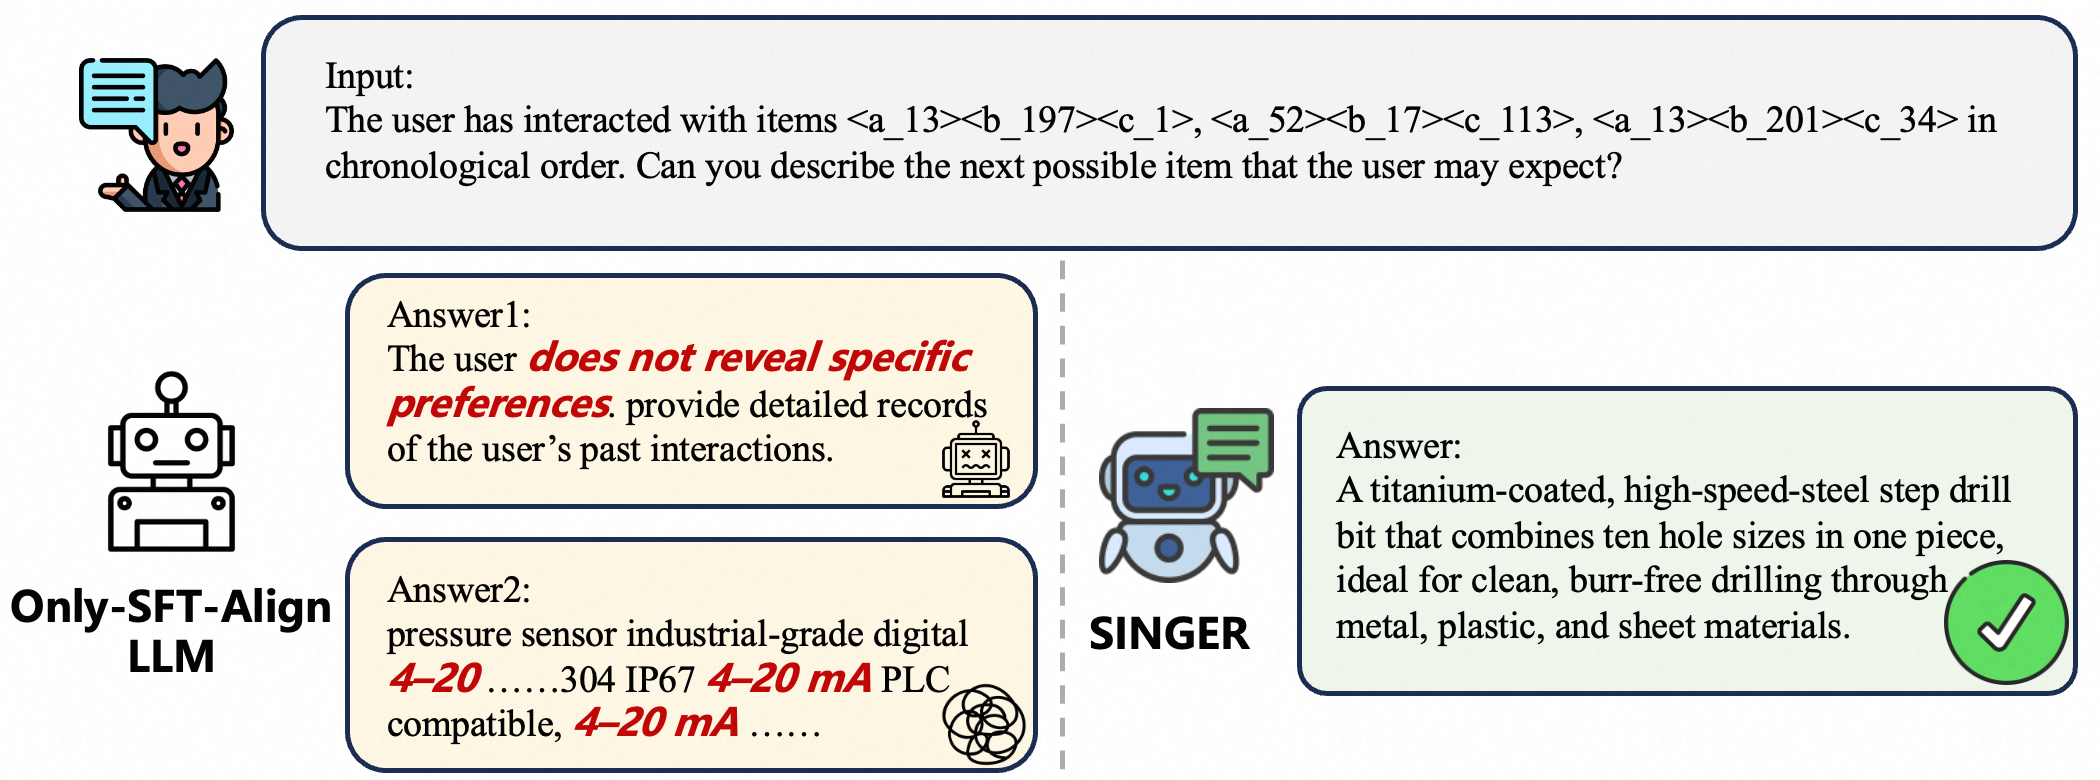
\includegraphics[width=1.0\textwidth]{figures/limited_understanding.png}
    \vspace{-10pt}
    \caption{Only-SFT-Align case study.  
The model is fed a SID-formatted interaction history and asked to describe the next item. The Only-SFT-Align LLM fails to interpret the SID tokens (Answer 1) or generates verbose, repetitive, and disordered text (Answer 2), underscoring the shallow alignment achieved by SFT alone. By contrast, MiniOneRec correctly understands the SID sequence and produces a concise, coherent item description.}
    \label{fig:superficial_align}
    \vspace{-10pt}
\end{figure}

We evaluate MiniOneRec on two public benchmark datasets \citep{amazon} and compare it with a wide range of leading traditional sequential recommenders, generative recommenders, and several recent LLM-based baselines. The results show that MiniOneRec consistently outperforms all competitors on standard recommendation metrics, confirming its effectiveness.
% \emph{A detailed survey of related work is deferred to Appendix~\ref{appendix:related_work}.}